\section{Abstract Factory}


\begin{figure}[htb]
	\caption{\label{fig_grafico}Estrutura do Abstract Factory}
	\begin{center}
	    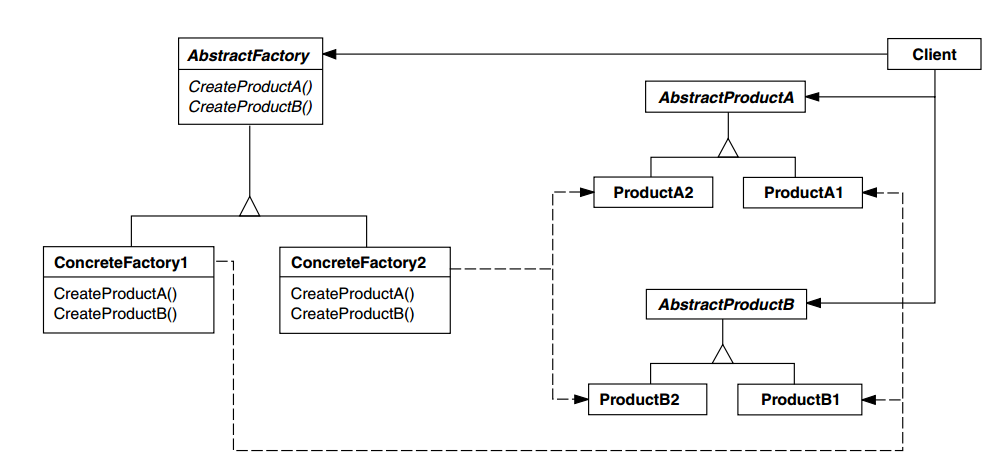
\includegraphics[scale=0.5]{5_padroes-contexto-funcional/5.1_criacionais/5.1.2_abstract-factory/diagram.png}
	\end{center}
\end{figure}

Exemplo Orientado a Objetos:

\begin{lstlisting}[caption={Abstract Factory Orientado a Objetos},label=oostrategy]
    

\end{lstlisting}

Contexto Funcional:

\begin{lstlisting}[caption={Abstract Factory Funcional},label=fpabfactory]
    
    

\end{lstlisting}